\hypertarget{saint-puxe9tersbourg-berceau-de-la-ruxe9volution}{%
\section{Saint-Pétersbourg, berceau de la
révolution}\label{saint-puxe9tersbourg-berceau-de-la-ruxe9volution}}

\emph{Mercredi 06 juin 2018}

C'est en train que nous avons rejoint Saint-Pétersbourg depuis Moscou.
Quatre heures, c'est le temps qu'on met à relier la ville nouvelle
fondée en 1703 par Pierre le Grand depuis la capitale actuelle. Nous y
avons passé presque une semaine et, au fil des balades à pied, découvert
une ville riche en palais colorés.

Comme un écho aux lourdes pierres de Baalbeck, on y trouve cette statue
équestre de Pierre le Grand :

\begin{figure}
\centering
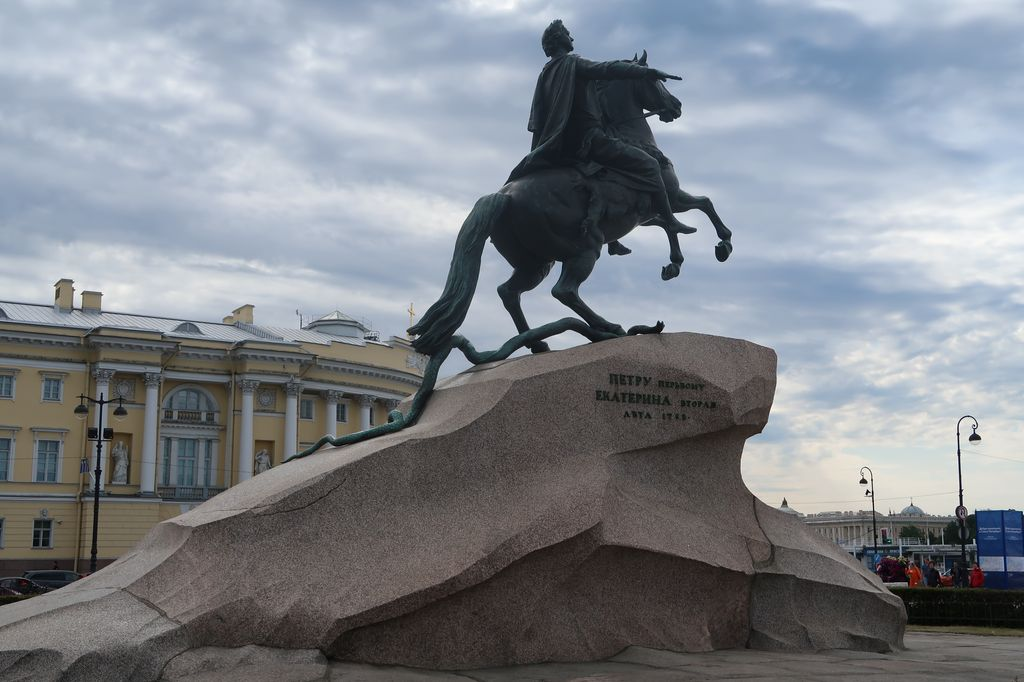
\includegraphics{images/20180606_pierre.JPG}
\caption{A notre droite, l'Ermitage, devant nous, la Neva et sous nous,
le granit.}
\end{figure}

On peut à ce sujet citer l'article de Jean-Pierre Adam justement déniché
lors de \href{/au-revoir-liban.html}{notre billet précédent}.

\begin{quote}
1.250.000 kilogrammes ! c'est le poids du formidable bloc de granite
(sic) que l'impératrice de Russie Catherine II (1762 à 1796) fit
transporter à Saint-Pétersbourg (aujourd'hui Leningrad) pour servir de
socle colossal à la statue équestre de Pierre le Grand. Il s'agit là
fort probablement de la plus grosse pierre jamais déplacée par l'homme,
une fois et demie le poids des blocs du trilithon.
\end{quote}

Mais Saint-Pétersbourg, après sa fondation comme nouvelle capitale de la
Russie des Tsars, a également été le siège de l'un des évènements les
plus marquants du XXème siècle (dixit notre ami Stanislav) : la
révolution d'octobre. Pour résumer, la prise de pouvoir des communistes
et le renversement du gouvernement provisoire après l'abdication des
Tsars en 1917 a entraîné la création de l'Union Soviétique à l'issue des
années de guerre civile qui ont suivi. Et c'est ici que cela a commencé.

\begin{figure}
\centering
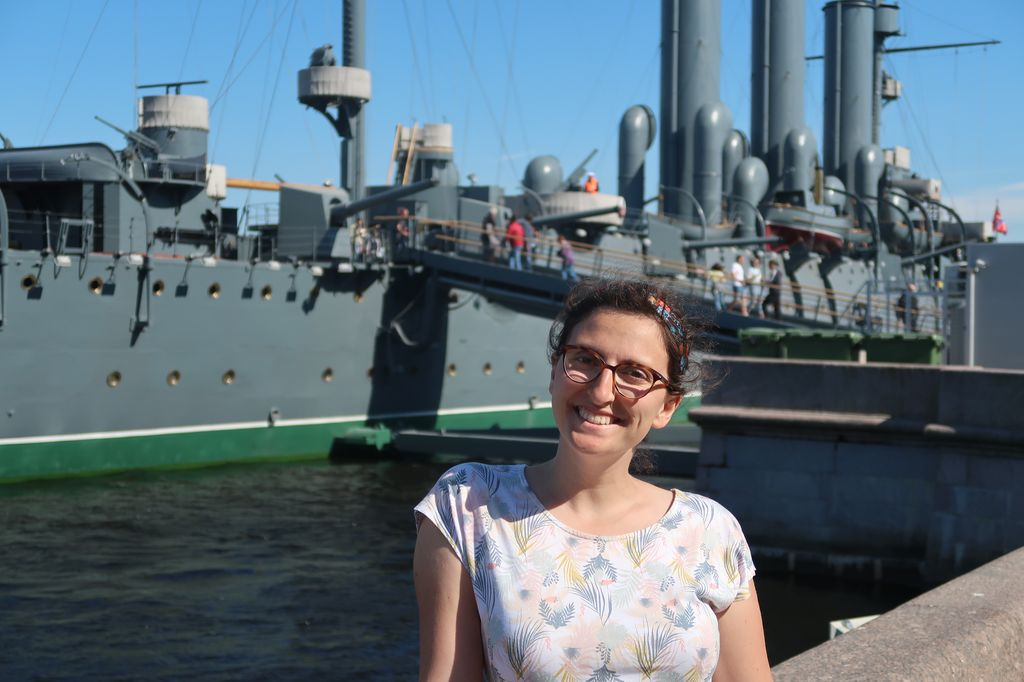
\includegraphics{images/20180606_Aurora.JPG}
\caption{Elida et le croiseur Aurora, contemporain aujourd'hui muet de
la révolution d'octobre, mais qui a donné le signal le jour J (en tirant
à blanc des coups de canon pour lancer l'assaut.}
\end{figure}

Avant de clore ce billet, il faut également mentionner que nous sommes
ici à une latitude bien plus élevée qu'à Paris. En conséquence, les
journées sont très longues et le soleil ne se couche presque pas à ce
moment de l'année. Cela rend d'autant plus agréable les nombreuses
balades par temps clair que nous avons pu faire. En particulier, nous
avons apprécié le lever des ponts de la ville, moment d'affluence
étonnant sur les berges et les eaux de la Neva à 1h30 du matin. En
principe rendu nécessaire par la navigation fluviale, c'est aussi l'une
des attractions constamment proposées aux touristes dans la ville. Mais
le charme opère, après une longue soirée à écouter un groupe de rock
russe sur la place de l'Ermitage...

\begin{figure}
\centering
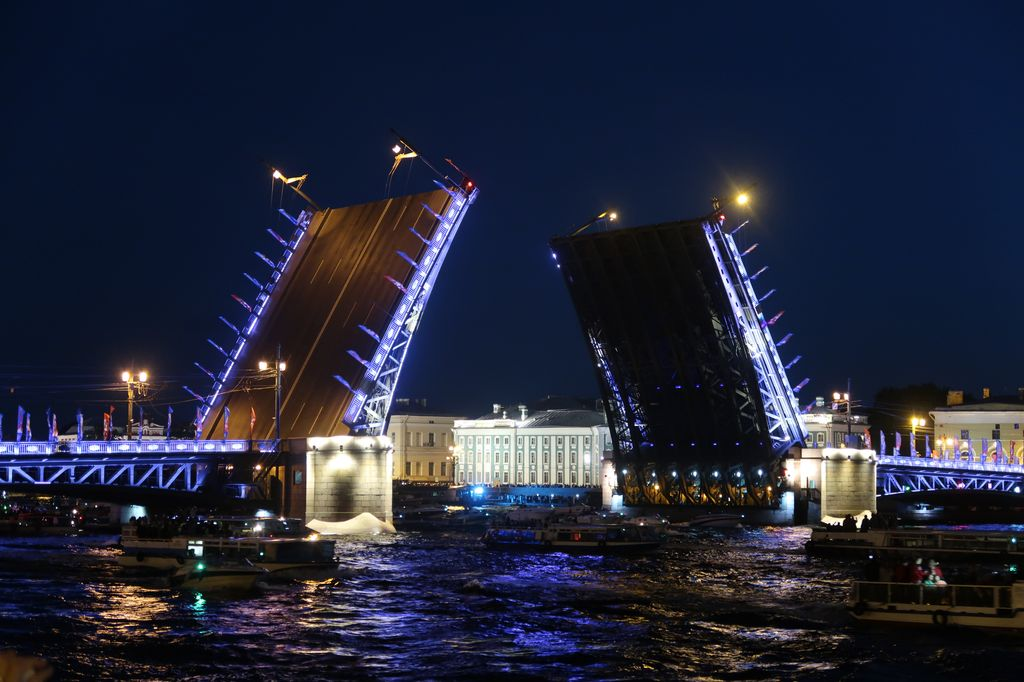
\includegraphics{images/20180606_pontpalais.JPG}
\caption{Le pont du palais vers 1h40 du matin.}
\end{figure}

Sur ce, nous vous donnons rendez-vous en Chine pour notre prochain
article !

\emph{Florian et Elida}
